\documentclass[a4paper,10pt]{report}\input{../0.Préambule/Préambule_cours_prof}\begin{document}

\newpage
\section*{Pyramides et cônes 1}
\addcontentsline{toc}{section}{Pyramides et cônes 1}

\begin{exer1}

\vspace{-8mm}

\includegraphics[scale=0.5]{../40.Image/Exo_Pyramide_et_cone_1.png}

\vspace{-3.58cm}\hspace{2cm}Nomme chaque solide représenté.
\vspace{3cm}
\end{exer1}

\begin{exer1}

\noindent \begin{minipage}{10.5cm}
Complète le tableau ci-dessous :
\begin{center}
\renewcommand{\arraystretch}{1.5}
\begin{tabularx}{\linewidth}{|>{\columncolor{exer1!20}\centering}p{3cm}|*{4}{>{\centering \arraybackslash}X|}}
\hline
\rowcolor{exer1!20} & $1$ & $2$ & $3$ & $4$\\\hline
Sommet &&&& \\\hline
Nature de la base &&&& \\\hline
Nom de la hauteur &&&& \\\hline
Hauteur &&&& \\\hline
Nombre d'arêtes &&&& \\\hline
Nombre de faces &&&& \\\hline
\end{tabularx}
\end{center}
\end{minipage}
\hspace{5mm}
\begin{minipage}{7cm}

\includegraphics[scale=0.6]{../40.Image/Exo_Pyramide_et_cone_2.png}
\end{minipage} 

\end{exer1}

\begin{exer1}
Un cône de révolution de hauteur $8,2$cm a pour base un disque de rayon $3,5$cm.

\noindent À main levée, dessine une représentation de ce cône de révolution en perspective cavalière puis code ton dessin.
\end{exer1}

\begin{exer1}
$SABCD$ est une pyramide régulière à base carrée telle que $SA=7,3$cm et $AB= 5$cm.

\noindent \begin{minipage}{11cm}
\begin{enumerate}[font=\color{exer1}]
\item Nomme le sommet et la base de cette pyramide.
\item Que représente le segment $[SH]$ pour la pyramide ? Justifie.
\item Indique, en centimètres, la longueur de chacune des arêtes de cette pyramide. Justifie.
\item Quelle est la nature du triangle $ADC$ ? Justifie. 

Construis-le en vraie grandeur.
\item Quelle est la nature du triangle $SAB$ ? Justifie. 

Construis-le en vraie grandeur.
\end{enumerate}
\end{minipage}
\hspace{5mm}
\begin{minipage}{5cm}
\begin{flushright}
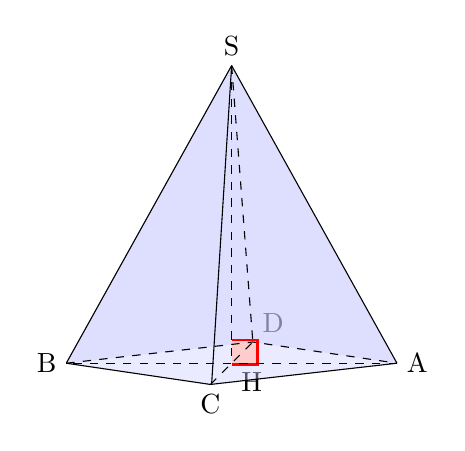
\begin{tikzpicture}[x=3cm,y=1.8cm,scale=0.7]
\tikzstyle{conefill} = [fill=blue!20,fill opacity=0.4] %couleur de fond
   
%coordonnées des sommets
\draw(0,3,0)node[above](S){S};
\draw(1,0,0)node[right](A){A};
\draw(-1,0,0)node[left](B){B};
\draw(0,0,1)node[below](C){C};
\draw(0,0,-1)node[above right](D){D};
\draw(0,0,0)node[below right](H){H};
   
%remplir les faces
\fill[conefill] (1,0,0)--(0,0,1)--(1,0,0)--(0,0,-1)--cycle; %base
\fill[conefill] (0,3,0)--(-1,0,0)--(0,0,-1); %arrière gauche
\fill[conefill] (0,3,0)--(-1,0,0)--(0,0,1); %avant gauche
\fill[conefill] (0,3,0)--(0,0,1)--(1,0,0); %avant droit
\fill[conefill] (0,3,0)--(1,0,0)--(0,0,-1); %arrière droit

\draw [line width=2pt,color=red] (0,0,0)--(0.15,0,0)--(0.15,0.22,0)--(0,0.22,0);
\fill[color=red!20] (0,0,0)--(0.15,0,0)--(0.15,0.22,0)--(0,0.22,0);

%tracer les arêtes
\draw (A.west)--(C.north)--(B.east);
\draw[dashed] (B.east)--(D.south west)--(A.west);
\draw (S.south)--(A.west);
\draw (S.south)--(B.east);
\draw (S.south)--(C);
\draw[dashed] (S.south)--(D.south west);
   
\draw [dashed] (S)--(0,0,0);
\draw[dashed] (A)--(B);
\draw[dashed] (C.north)--(D.south west);  
\end{tikzpicture}
\end{flushright}
\end{minipage}
\end{exer1}

\begin{exer1}
Une pyramide régulière de hauteur $7$cm a pour base un carré de côté $5$cm.
\begin{enumerate}[font=\color{exer1}]
\item A main levée, dessine une représentation de cette pyramide en perspective cavalière puis code ton dessin.
\item Construis à la règle une représentation en perspective cavalière de cette pyramide.
\end{enumerate}
\end{exer1}

\begin{exer1}
Un tétraèdre régulier est une pyramide dont toutes ses faces sont des triangles équilatéraux.

\medskip
\noindent Trace le patron d'un tétraèdre régulier d'arête $5,5$cm.
\end{exer1}

\begin{exer1}
Pour calculer la mesure de l'angle du développement d'un cône, on utilise la formule : $\widehat{a}=\dfrac{360 \times R}{g}$ où $R$ est le rayon du disque de base et $g$ la longueur de la génératrice du cône.
\begin{enumerate}[font=\color{exer1}]
\item Calcule la mesure de l'angle du développement du cône représenté ci-contre où $SN=6,5$cm et $AN=2,6$cm.
\item Trace le patron de ce cône.
\end{enumerate}
\end{exer1}

\begin{exer3}

\noindent \begin{minipage}{5cm}
\definecolor{qqwuqq}{rgb}{0.,0.39215686274509803,0.}
\begin{tikzpicture}[line cap=round,line join=round,>=triangle 45,x=1.0cm,y=1.0cm,scale=0.7]
\clip(-0.2,1.5) rectangle (7.5,9.5);
\draw [shift={(2.84,4.84)},line width=1.2pt,color=qqwuqq,fill=qqwuqq,fill opacity=0.1] (0,0) -- (-67.78240573048168:0.5514963294579209) arc (-67.78240573048168:157.78240573048168:0.5514963294579209) -- cycle;
\draw [shift={(2.8333333333333335,4.833333333333333)},line width=1.2pt]  plot[domain=-1.18018928309721:2.7509856098921066,variable=\t]({1.*3.0641293851417064*cos(\t r)+0.*3.0641293851417064*sin(\t r)},{0.*3.0641293851417064*cos(\t r)+1.*3.0641293851417064*sin(\t r)});
\draw [shift={(2.8333333333333335,4.833333333333333)},line width=1.2pt,color=black,fill=blue,fill opacity=0.1]  (0,0) --  plot[domain=-1.18018928309721:2.7509856098921066,variable=\t]({1.*3.0641293851417064*cos(\t r)+0.*3.0641293851417064*sin(\t r)},{0.*3.0641293851417064*cos(\t r)+1.*3.0641293851417064*sin(\t r)}) -- cycle ;
\draw [shift={(6.,8.)},line width=0pt,color=red!10,fill=red,fill opacity=0.1]  (0,0) --  plot[domain=-2.356194490192345:3.5451367038651966,variable=\t]({1.*1.4142135623730951*cos(\t r)+0.*1.4142135623730951*sin(\t r)},{0.*1.4142135623730951*cos(\t r)+1.*1.4142135623730951*sin(\t r)}) -- cycle ;
\draw [shift={(6.,8.)},line width=0pt,color=red!10,fill=red,fill opacity=0.1]  (0,0) --  plot[domain=3.5451367038651966:3.9269908169872414,variable=\t]({1.*1.414213562373095*cos(\t r)+0.*1.414213562373095*sin(\t r)},{0.*1.414213562373095*cos(\t r)+1.*1.414213562373095*sin(\t r)}) -- cycle ;
\draw [line width=1.2pt] (6.,8.) circle (1.4142135623730951cm);
\draw [line width=1.2pt] (6.,8.)-- (2.84,4.84);
\draw [line width=1.2pt] (0.,6.)-- (2.84,4.84);
\draw [line width=1.2pt] (2.84,4.84)-- (4.,2.);
\begin{scriptsize}
\draw [color=black] (6.,8.)-- ++(-2.5pt,0 pt) -- ++(5.0pt,0 pt) ++(-2.5pt,-2.5pt) -- ++(0 pt,5.0pt);
\draw[color=black] (6.125380850950418,8.34780434436207) node {\large{$O$}};
\draw[color=black] (5.206220301853884,8.108822601596971) node {\large{$3$cm}};
\draw [color=black] (0.,6.)-- ++(-2.5pt,0 pt) -- ++(5.0pt,0 pt) ++(-2.5pt,-2.5pt) -- ++(0 pt,5.0pt);
\draw[color=black] (0.18760370378680385,5.480023431180885) node {\large{$B$}};
\draw [color=black] (4.,2.)-- ++(-2.5pt,0 pt) -- ++(5.0pt,0 pt) ++(-2.5pt,-2.5pt) -- ++(0 pt,5.0pt);
\draw[color=black] (3.4965816805343293,1.8217644457766815) node {\large{$A$}};
\draw [color=black] (2.84,4.84)-- ++(-2.5pt,0 pt) -- ++(5.0pt,0 pt) ++(-2.5pt,-2.5pt) -- ++(0 pt,5.0pt);
\draw[color=black] (2.5038882875100716,4.52409646012049) node {\large{$S$}};
\draw[color=black] (3.51496489151626,6.638165723042517) node {\large{$5$cm}};

\end{scriptsize}
\end{tikzpicture}
\end{minipage}
\begin{minipage}{11.4cm}
\begin{enumerate}[font=\color{exer3}]
\item Nomme une génératrice de ce cône. Calcule la valeur exacte de la circonférence du grand cercle ayant pour rayon la longueur de cette génératrice et pour centre le point $S$.
\item Détermine la valeur exacte de la circonférence du cercle de base.
\item Quelle est la valeur exacte de la longueur de l'arc de cercle $\widehat{(AB)}$ ? Justifie.
\item On admet qu'il y a proportionnalité entre la mesure de l'angle au centre $\alpha =\widehat{(BSA)}$ et la longueur de l'arc $AB$ qui l'intercepte. Calcule $\alpha$ en utilisant le tableau suivant :
\begin{center}
\renewcommand{\arraystretch}{1.5}
\begin{tabularx}{\linewidth}{|>{\columncolor{exer3!20}\centering}p{4cm}|*{2}{>{\centering \arraybackslash}X|}}
\hline
\rowcolor{exer3!20} & Longueur & Mesure de l'angle \\\hline
Grand Cercle && $360$\degre \\\hline
Arc de cercle && $\alpha$ \\\hline
\end{tabularx}
\end{center}
\item A partir des résultats précédents, construis en vraie grandeur le patron de ce cône.
\end{enumerate}
\end{minipage}
\end{exer3}

\begin{exer3}

\medskip
\noindent \begin{minipage}{5.5cm}
\begin{center}
\begin{tikzpicture}[general,scale=0.7]
\draw(1,1.5) node[below] (A){$A$};
\draw(5,1) node[below] (B){$B$};
\draw(7,2) node[right] (G){$G$};
\draw (1,5.5) node[left] (D){$D$};
\draw(5,5) node[above] (C){$C$};
\draw(7,6) node[right] (F){$F$};
\draw(3,6.5) node[above] (E){$E$};
\draw(3,2.5) node[above left] (H){$H$};
\draw(4,3.75) node[above] (O){$O$};
\draw (1,1.5)-- (5,1)-- (5,5)--(1,5.5)--cycle;
\draw (1,5.5)--(3,6.5)--(7,6)--(5,5);
\draw (7,6)--(7,2)--(5,1)--(5,5);
\draw [dashed] (7,2)--(3,2.5);
\draw [dashed] (3,2.5)-- (1,1.5);
\draw [dashed] (3,2.5)-- (3,6.5);
\draw (1,5.5)--(5,5)--(7,6);
\draw [color=red, dashed] (A.north)--(F.west);
\draw [color=blue, dashed] (H.south east)--(O.south);
\draw [color=blue, dashed] (G.west)--(O.south);
\draw [color=blue, dashed] (B.north)--(O.south);
\draw [color=red, dashed] (D.east)--(F.west);
\end{tikzpicture}
\end{center}
\end{minipage}
\begin{minipage}{11cm}
\begin{enumerate}[font=\color{exer3}]
\item $ABCDEFGH$ est un cube. $O$ est le milieu de $[AF]$.
Quelle est la nature du triangle $DFA$ ? Justifier.
\item Sachant que $AD=6$cm, donnez la valeur approchée par excès au mm près de $DF$,$ AF$ et $AO$.
\item Expliquez pourquoi $AO=OB=GO=HO$. Quelle est la nature du solide $OABGH$ ?
\item Construisez un patron de $OABGH$ puis découpez-le et collez-le pour obtenir la pyramide.
\item Faites cinq autres exemplaires de cette pyramide. Avec les six pièces ainsi constituées, essayez de reformer le cube $ABCDEFGH$.
\end{enumerate}
\end{minipage}

\begin{enumerate}[font=\color{exer3}]
\setcounter{enumi}{5}
\item Construisez un patron du cube $ABCDEFGH$, collez chacune des pyramides sur une face du cube. Assemblez ensuite le cube en plaçant les pyramides à l'extérieur.
\item Le solide obtenu s'appelle un dodécaèdre rhombique car chacune de ses faces est un losange. Combien a-t-il de faces ?
\item Construisez un patron du dodécaèdre rhombique et assemblez le directement.
\end{enumerate}
\end{exer3}
\end{document}